\chapter{Систематизация и анализ общих проблем}\label{ch:ch1}

\section{Основные определения}\label{sec:ch1/sec1}

В начале главы необходимо привести основные определения терминов, которые будут использоваться в рамках данного исследования в первой главе. Приведем описание самых основных определений.

Автоматизированные системы управления - комплекс аппаратных и программных вычислительных машин, а также персонала, цель которого заключается в обеспечении автоматизированной работы технологического процесса.

Нейронные сети - искусственная модель математической концепции обработки информации, проектируемая статистическими методами обработки информации на основе наблюдений принципов работы нейронов.

Нечеткая логика - логика, основанная на относении того или иного объекта к некоторой численной мере согласно функциям принадлежности.

Более подробно все остальные определения изложены в разделе Словарь терминов.

\section{Определение объекта исследования}\label{sec:ch1/sec2}
Объектом исследования выступает: модель поддержки принятия решений для проектирования автоматизированной системы управления, формализованная посредством сетевой модели представления данных для отбора альтернатив с помощью методологии на основе моделей машинного обучения.

Методом построения автоматизированной системы управления выступает система поддержки принятия решений в проектировании архитектуры автоматизированной системы управления технологическими процессами(АСУТП) и производствами (АСУП), а также технической подготовкой производства (АСТПП) ит. д. с использованием адгоритмов поддержки принятия решений.

Под проектированием архитектуры подразумеваются следующие действия:
\begin{enumerate}
    \item  поиск, анализ и подбор инструментов построения,
    \item  поиск, анализ и подбор парадигмы организации и реализации информационно-вычислительной части построения автоматизированной системы управления,
    \item  поиск, анализ и подбор серверной части организации работы автоматизированной системы управления,
    \item  проектирование организации работы  вычислительной техники и программных средств, предназначенных для управления, хранения, представления информации в локальной вычислительной сети для рабочих мест и других сетевых устройств,
    \item  проектирование организации работы инфокоммуникационной техники и программных средств, предназначенных для управления, хранения, представления информации в локальной вычислительной сети для рабочих мест и других сетевых устройств.
\end{enumerate}

Таким образом, в работе исследуется модель поддержки принятия решений проектирования архитектуры автоматизированной системы управления. 
При проектировании архитектуры автоматизированной системы управления рекомендуется соблюдать требования, сформулированные в стандарте\cite{ACSSt}.

В данной работе рассматривается вопрос относительно проектирования модели поддержки принятия решений для построения архитектуры программного обеспечения автоматизированной системы управления.

При проектированнии системы поддержки принятия решений для проектирования устойчивой архитектуры автоматизированных систем управления следует выделить следующие основопологаюшие объекты:
\begin{enumerate}
    \item модель,
    \item объект,
    \item базовая модель,
    \item модель данных,
    \item информационная модель,
    \item организация данных в системах,
    \item инфологическая модель,
    \item модель представления данных,
    \item нормализация,
    \item форма,
    \item информационная нагрузка,
    \item информационный поток данных,
    \item информационный объем данных,
    \item гарантия доставки сообщений,
    \item производительность процесса, 
    \item производительность системы,
    \item ошибки работы системы,
    \item время обслуживания,
    \item объекты, структурирующие данные,
    \item процессы,
    \item ресурсы,
    \item состояния.
\end{enumerate}

Модель - термин произошедший от латинского слова "modulus", который представляет собой некоторую абстрактную модель представления системы, которое создается с целью анализа  работы системы, а также получения качественных и количественных характеристик работы системы.

Объект - некоторый элемент, представляющийся в системе, как совокупность свойств элемента, которые выступают, как единое целое.

Базовая модель - это модель, которая содержит описаний функций, процессов, объектов, правил для структурирования данных в конкретной реализации БД.

Модель данных - результат структурирования данных посредством выражения абстрактной модели объекта данных.

Информационная модель данных - модель представления данных в виде чертежей, схем, таблиц, и т.д.

Организация данных в системе - представление данных в виде структурированной системы с описанием характеристик каждого объекта информации.

Инфологическая модель - модель отображения данных в виде информационно-логического представления.

Модель представления данных - представление информации в системе, с помощью некоторой логической структуры. Самыми распространенными моделями являются следующие: иерархическая, сетевая, реляционная,  постреляционная, многомерная, объектно-ориентированная.

Нормализация - процесс приведения данных к некоторому формализованному виду посредством выражения через некоторые формы и связи между формами. На начальном этапе определяются основополагающие отношения между объектами в предоставленной конкретной области применения системы. На следующем этапе производится декомпозиция сложных объектов. На заключительном этапе  производится декомпозиция неключевых атрибутов.

Форма - стурктурированный объект, представленный в виде таблицы.

Информационная нагрузка - нагрузка, поступающая от пользователей или количество информации в виде потребляемого трафика от каждого пользователя, системы или устройства получающей информацию от системы. 
 
Информационный поток - поток событий в виде информационных транзакций, происходящих за единицу времени.

Информационный объем - общий поток информации, приходяшийся на процесс.

Гарантия доставки сообщений - риск потерия сообщений.

Производительность процесса - количество операций, завершенных с успехом за единицу времени, по отношению ко всем операциям.

Производительность системы - общее суммарное значение всех процессов, завершенных с успехом за едицину времени, по отношению ко всем операциям в процессе.

Ошибки работы системы - процессы, которые ведут к ошибочным состояниям работы системы.

Время обслуживания - время, за которое производится то или иное действие внутри системы. Например, время обработки документа или отлик на действие пользователя. 

Объекты, структурирующие данные - объекты системы, которые вопроизводят информацию для которой необходимо подобрать структуру данных для хранения, передачи, обработки.

Процесс - отношение между объектами, выраженные посредством некоторых действий или характеров связи (ассоциация, обобщение, агрегация, композиция).

Ресурс - ресурс, необходимый для работы программного обеспечения (память, процессор, диск, сеть, трудовые кадры, бюджет).

Состояние - отображение наблюдения за результатом работы объекта или процесса за некоторый отрезок времени в системе.

\subsection{Характеристика объекта исследования}\label{sec:ch1/sec2/sec2}
В работе обсуждается вопрос проектирования модели поддержки принятия решений для проектирования архитектуры программного обеспечения системы. 
Таким образом, в работе решение задачи - проектирования системы поддержки принятия решений для построения рекомендаций по проектированию автоматизированной системы управления - сводится к задаче проектирования программного обеспечения автоматизированной системы управления посредством анализа применения альтернатив, принятия решений о реализации и сравнения методологий.

Автоматизированная система управления, согласно международному стандарту\cite{ACSSt}, должна обладать следующими свойствами:
\begin{enumerate}
    \item  полнота,
    \item  надежность систем (в том числе восстанавливаемость, наличие средств выявления ошибок),
    \item  адаптируемость к входным нагрузкам,
    \item  модифицируемость или возможность обновления при необходимости,
    \item  модульность построения частей системы или всей системы в целом, 
    \item  удобство эксплуатации, не требующая больших затрат в обучении персонала.
\end{enumerate}  

Для разработки модели поддержки принятия решений при проектировании программного обеспечения следует дать характеристику методологии проектирования. Методолология проектирования состоит из следующих аспектов, в которых рассматривается модель поддержки принятия решения:
\begin{enumerate}
    \item  определение объектов данных, которые будут реализованы в базе данных,
    \item  определение связей между объектами, которые будут реадизованы в базе данных,
    \item  определение логики действия с объектами данных на основании типовых сценариев использования,
    \item  определение количества пользователей, среднюю нагрузку по запросам к системе
    \item  определение количества информации, проходящей по потокам,
    \item  определение конкретной аппаратно-вычислительной среды развертывания программного обеспечения,
\end{enumerate}
На начальном этапе проектирования определяются цели проекта. Цели проекта - взаимосвязанные функционально-технические решения, обеспечивающие выполнения конкретных задач и функций проекта в течении всего времени эксплуатации. На момент определения целей требуется конкретизировать следующие аспекты реализации:
\begin{enumerate}
    \item  требования к функционалу системы,
    \item  требования к пропускной способности,
    \item  требования к отклику и времени обработки информации,
    \item  требования к обработке отказов и исключительных ситуаций,0
    \item  требования к уровню безопасности,
    \item  требования к эксплуатации и поддержки работы системы.
\end{enumerate} 
Таким образом, модель поддержки принятий решений должна предоставлять альтернативы методологий проектирования на основе анализа целей, процессов, объектов и требований к проектированию программного обеспечения.

\section{Анализ проблем проектирования автоматизированных систем}\label{sec:ch1/sec3}
Рассмотрим класс так называемых автоматизированных систем. Дадим определение понятия автоматизированной системы - это система, нагруженная обработкой данных, где основными проблемами являются: качество данных, степень их сложности, скорость изменений. Такие системы состоят из взаимосвязанной совокупности подразделений организации комплекса средств автоматизации деятельности технологического предпртиятия, производства или любой другой деятельности, подразумевающей управление производственным процессом. Это человеко-машинная система, предназначенная для сбора, обработки и хранения данных информации, необходимой для управления производственным процессом~\cite{Ref1, Ref2, Ref3, Ref4,Ref5,Ref6,Ref7, Ref8, Ref9, Ref10,Ref11,Ref12}.

Введем следующие основополагающие понятия для данной работы:
\begin{enumerate}
    \item  надежность;
    \item  масштабируемость;
    \item  удобство сопровождения.
\end{enumerate}


Основной проблемой современных систем является обработка сложного объема данных, а также скорости его изменения. Автоматизированные данными приложения (автоматизированные системы) зачастую состоят из стандартного набора блоков. Представим типовой перечень функциональности:
\begin{enumerate}
    \item  хранение данных, чтобы в дальнейшем можно было эти данные найти;
    \item  запоминание результатов высокоемкий ресурсозатратных операций для ускорения чтения (кэш);
    \item  предоставление пользователям возможности поиска данных по ключевому слову, фильтрации по некоторым параметрам;
    \item  отправление сообщений другим процессам для асинхронной обработки (потоковой обработки);
    \item  дробление данных в некоторые моменты времени.
\end{enumerate}

\section{Определение проблем проектирования автоматизированной систем управления}\label{sec:ch1/sec4}

Проблема проектировани автоматизированной системы управления довольно распространенная проблема, ввиду принятия решений человеком, что может спровоцировать ошибки проектирования из-за недостаточно полного восприятия полного набора объетов, участвующих в системе.
Проблемы проектирования могут возникать по следующим причинам:
\begin{enumerate}
    \item неверно определенные цели системы автоматизированного управления,
    \item неверное понимание циркуляции информационных потоков в системе,
    \item неверное понимание сценариев развертывания, сценариев использования системы,
    \item неверное понимание функционала объектов, участвующих в системе,
    \item неверное понимание и расчет параметров нагрузки на систему,
    \item неверное понимание количества вычилительных устройств, участвующих в системе,
    \item проблемы с нехваткой специализованных кадров на местах проектирования архитектуры программного обеспечения.
\end{enumerate}

Для того, чтобы создать модель архитектуры автоматизированной системы управления на уровне производства необходимо сформировать требования экспуатации к такой системе. Одним из основных методов к созданию модели автоматизированных систем управления является построение структуры работы информационных потоков на некотором технологическом процессе производства. Главным приниципом создания модели архитеткру является анализ существующей системы управления с точки зрения информационных потоков, анализ деятельности людей и сценариев обмена информационными потоками в процессе взаимодействия. Данная работа над моделью предполагает рассмотрение конкретных участков производства в виде отдельных компонент, синтезируя которые, можно выделить структурную модель анализа вариантов обмена информационными потоками в структуре предприятия~\cite{Ref13, Ref14, Ref15, Ref16,Ref17,Ref18,Ref19, Ref20, Ref21, Ref22,Ref23,Ref24}.

Структурная модель должна содержать оба основных элемента, а именно: производственные мощности и средства организации материального потока. Комбинируя эти элементы, исследователи и организаторы системы делят всю структуру предприятия на буферную и технологическую части. При этом охватываются все виды деятельности - от получения сырья до передачи готовой продукции покупателю. Основной критерий, отличающий буферные и технологические зоны, сосредоточен в вопросе: находится ли предмет труда в стационарном состоянии или он приведен в движение? Получив ответ на этот вопрос, далее определяют, какие конкретно данные должны быть собраны, обработаны и переданы для обеспечения оптимального управления материальным потоком.

Информация является одним из главных типов ресурсов, которые необходимы менеджеру любого класса. Роль этого ресурса постоянно возрастает по двум основным причинам:
\begin{enumerate}
    \item  глобализации экономики и управления (производство становится комплексным и международным);
    \item  более обширных требований к организованности ресурсов, предъявляемых автоматизацией.
\end{enumerate}

Системный подход опирается на предварительную оценку определения места информационного ресурса среди других видов ресурсов организации любого типа.
Любая организация имеет пять основных типов ресурсов, которыми она должна управлять как соответствующими потоками:
 \begin{enumerate}
    \item  человеческие ресурсы;
    \item  материальные ресурсы;
    \item  технические ресурсы(включая оборудование и энергию);
    \item  финансовые ресурсы;
    \item  информационные ресурсы(включая данные);
\end{enumerate}
В научной литературе существует и широко используется представление процесса управления как процесс обработки информации. Таким образом, при разработке информационного обеспечения учитываются общие свойства систем:
\begin{enumerate}
    \item  система представляется в виде набора компонентов;
    \item  составные компоненты логически взаимосвязаны между собой;
    \item  система имеет связь с внешней средой~\cite{Ref25, Ref26, Ref27, Ref28,Ref29,Ref30,Ref31, Ref32, Ref33, Ref34,Ref35,Ref36}.
\end{enumerate}


\subsection{Проблема проектирования устойчивой архитектуры программного обеспечения автоматизированной системы управления}\label{subsec:ch1/sec4/sub1}

Проблемы проектирования устойчивой архитектуры является наиболее актуальной проблемой на сегодняшний день в мире разработки программного обеспечения для всех типов систем. В связи с расширяющимся спектром автоматизации действий человека, растущим спросом на разработку программного обеспечения для оптимизации производства, а также сложностью технического и технологического исполнения задачи проектирования устойчивой к масштабирования и росту нагрузки архитектуры программного обеспечения растет с каждым годом.
Несмотря на появление новых технологий, вычислительных средств и средств разработки проектирование человеко-машинных средств автоматизации по прежнему основано на принципах, сформивовавшхся в эпоху приборных панелей с мнемосхемами и приборными пультами.С увеличение потоков информации растет и необходимость в разработке новых принципов и методологий проектирования архитектуры программного обеспечения автоматизации систем управления. С увеличением требований к безопасности растет необходимость проектирования программного обеспечения автоматизированных систем управления с использованием современных средств и методологий защиты информации и оборудования от кибератак и утечек~\cite{Ref60, Ref61, Ref62, Ref63,Ref64,ISA}. 

\subsection{Проблема масштабирования архитектуры программного обеспечения автоматизированной систему управления}\label{subsec:ch1/sec4/sub2}
Современные стандарты проектирования составлялись во времени более ограниченных факторов проектирования программного обеспечения:
\begin{enumerate}
    \item  менее слабыми вычислительными ресурсами,
    \item  высокой трудоемкостью работ,
    \item  высокой стоимостью оборудования для обеспечения автоматизации,
    \item  наличие только теоретических моделей сложных систем,
    \item  отсутствие возможности верификации надежности или устойчивости работы спроектированных сложных систем.
\end{enumerate}
В работах прошлых лет основным тезисом ненадежности автоматизации считается следующий постулат: человек не очень надежен, но способен действовать в сложноформализуемых ситуациях, в то время, как машина не способна принимать решения в условиях семантической ограниченности\ifnumequal{\value{bibliosel}}{0}{\cite{GolKos, Inag, Anohin, KanSor}}.
Благодаря таким ограничениям вопросы масштабирования архитектуры программного обеспечения не рассматривались системно.

\subsection{Проблема обеспечения доступности, целостности, конфиденциальности информации при проектировании архитектуры программного обеспечния автоматизированной системы управления}\label{sec:ch1/sec4/sub5}

Основой работы программного обеспечения в штатном режиме является ее безопасность. Перечислим фундаментальные критерии безопасности, которые необходимо соблюдать при проектировании архитектуры:
\begin{enumerate}
    \item   Доступность т.е. обязательство, что программное обеспечение будет доступно пользователям. Пользователи будут иметь доступ к программному обеспечению, к его активам, ресурсам и функционалу, работа программного обеспечения должна обеспечивать необходиму для пользователя производительность. В доступность также включается обеспечение безопасности от злонамеренного неавторизованного доступа.
    \item  Целостность - это обязательство, что информация остается неизменной, корректной, аутентичной.
    \item  Конфиденциальность - обеспечение доступа к информации только тем людям, кто имеет право доступа к информации и авторизованн это делать.
\end{enumerate}

При проектировании программного обеспечения необходимо обеспечивать гарантированность выполнения сервисов безоапсности путем разработки организационной схемы политики безопасности работы программного обеспечения. Для обеспечения гарантированности выполнения должна проводится работа по анализу рисков для информационных активов\cite{Ref1}.

\section{Анализ проблем проектирования автоматизированных систем}\label{sec:ch1/sec5}

Проведем анализ проблем проектирования автоматизированных систем и приведем теоретическое обоснование проведенного анализа с точки зрения теоретико-множественного и теоретико-информационного аспектов.

\subsection{Теоретико-множественный анализ задачи проектирования архитектуры автоматизированных систем управления}\label{sec:ch1/sec5/sub1}

Объектом познания является система проектирования архитектуры автоматизированных систем управления. Система обладает следующими свойствами:
\begin{enumerate}
    \item  организованность,
    \item  функциональность,
    \item  доступность,
    \item  конфиденциальность,
    \item  целостность.
\end{enumerate}

Каждому свойству объекта соответствует переменная, с помощью которой отображается проявление свойства через множество пространства состояний, принимаемых переменной.  

\begin{equation}
    \label{eq:equation1}
    D: S_i = [S_{i,j}], \rightarrow X_i = [X_{i,j}]
\end{equation}

где $i = \{1,...,N\}$, 

$j = \{1,...,M\}$,

$S_i$ - i-ое свойство объекта,

$X_i$ - переменная.
Представим систему в виде множества:

\begin{equation}
    \label{eq:equation2}
    S = (X,T,R,Z)
\end{equation}

где $X$ — множество переменных, 

$T$ — множество параметров, 

$R$ — отношения на множествах $X$ и $T$, 

$Z$ — цель исследований.

Отношения между переменными задаются в виде отношения полезности использования и упорядоченности перемененных на множестве параметров. Таким образом отношения объединяют структурно-динамические свойства системы.

Структурные отношения показывают характер взаимодействия или зависимости между объектами, т.е. каким образом происходит взаимоотношение между объектами. Динамические свойства определяют нагрузку на объекты и устойчивость отношений между объектами.

Каждое значение переменной изменяется на множестве переменных в некоторой области значений заданной множеством физически различных значений:

\begin{equation}
    \label{eq:equation3}
    <X> = {x_1, x_2, ..., x_n}, n \in {R}  
\end{equation}

Зафиксированное знаенчие всех возможных состояний системы задается в виде вектора состояний:
\begin{equation}
    \label{eq:equation4}
    C_i = [\alpha_{i,k_i}, X_i], i \in N 
\end{equation}

Множество всех возможных векторов состояний образует полное множество состояний.

Пусть вектор $<X>$ отражает свойства объекта:
\begin{equation}
    \label{eq:equation5}
    <X> = <X_1, X_2, ..., X_n> 
\end{equation}

где $n \in D$ - размерность вектора $<X>$ определяется размерностью пространства свойств объекта.

Пусть вектор $<X>$ зависит от набора параметров системы $T^i$, где каждое значение $T^i$, $i\in \{1,2,...,P\}$ отражает конкретный параметр объектов в системе:
\begin{equation}
    \label{eq:equation6}
    <T> = <T^1, T^2, ..., T^n> 
\end{equation}

Значение  матриц-векторов параметров приведены в Таблице~\cref{tab:T:param}.
\begin{table}
    \centering
    \captionsetup{justification=centering} % выравнивание подписи по-центру
    \caption{Основные матрицы параметров}\label{tab:T:param}
    \begin{tabular}{llc}
        \toprule
        Абревиатура  & Название   \\
        \midrule
        <T^1_{n_1,m_1}>    & \verb|матрица отношений между объектами|\\
        <T^2_{n_2,m_2}>   & \verb|матрица атрибутов объектов|\\
        <T^3_{n_3,m_3}>   & \verb|матрица поведения объектов|\\
        <T^4_{n_4,m_4}> & \verb|матрица информационной нагрузки|\\
        <T^5_{n_5,m_5}>      & \verb|матрица пропускной способности|\\
        \bottomrule
    \end{tabular}
\end{table}

Каждому вектору свойств соответсует своя суперпозиция векторов-матриц параметров соответственно:
\begin{equation}
    \label{eq:equation7}
    <X_k> = f(g(\cup^P_{i=1}T^i_{n_i,m_i})), k \in \{1, 2, ..., D\}
\end{equation}

Значение векторов свойств приведены в Таблице~\cref{tab:X:prop}.
\begin{table}
    \centering
    \captionsetup{justification=centering} % выравнивание подписи по-центру
    \caption{Основные вектора свойств, $i \in \{1, 2, ..., D\}$}\label{tab:X:prop}
    \begin{tabular}{llc}
        \toprule
        Абревиатура  & Название   \\
        \midrule
        <X^1_i>    & \verb|вектор целостности|\\
        <X^2_i>   & \verb|вектор конфиденциальности|\\
        <X^3_i>   & \verb|вектор доступности|\\
        <X^4_i> & \verb|вектор организованности|\\
        <X^5_i>      & \verb|матрица функциональности|\\
        \bottomrule
    \end{tabular}
\end{table}
Тогда целевая функция примет вид:
\begin{equation}
    \label{eq:equation8}
    F(\varphi(R(x)) = \varphi(f(g(\cup^P_{i=1}T^i_{n_i,m_i}))) \rightarrow opt
\end{equation}

где $x$ - обобщенный вектор свойств системы,

$R$ - оператор отношения,

$\varphi$ - функция отображения определения полезности суперпозиции параметров и свойств.

Пространство состояний параметров принадлежат вещественному полю и ограничены на полном множестве состояний.


\subsection{Теоретико-информационный анализ задачи проектирования архитектуры автоматизированных систем управления}\label{sec:ch1/sec5/sub2}
Пусть архитектура программного обеспечения автоматизированной системы управления является некоторой абстракцией модели сопряжения датчиков, устройств ввода-вывода, измерительных преобразователей, программируемых логических контроллеров, компьютеров, интерфейсов, протоколов, промышленных сетей, исполнительных устройств, драйверов, каналов передачи информации. 
Тогда, поток входящих заявок на обслуживание образуют, так называемый, случайный поток заявок. Обслуживание заявок происходит также за некоторое случайное время, интервал между событиями является случайной величиной. В качестве показателей используются: 
\begin{enumerate}
\item  среднее число заявок, обслуживаемых в единицу времени; 
\item  среднее число заявок в очереди; среднее время ожидания обслуживания; 
\item  вероятность отказа в обслуживании без ожидания; 
\item  вероятность превышения числа заявок определенного значения. 
\end{enumerate}

Таким образом, поведение потока будет описываться стационарным пуассоновским потоком с отсутствием последействия. Следует найти решение о степени приближения плотности распределения времени между событиями поступления и обработки заявок к плотности распределения интервалов в простейшем потоке и составить модель архитектуры для обслуживания систем с учетом стационарной случайной нагрузки на ресурсы автоматизированной системы. 
Рассмотрим параметрический критерий, основанный на следующем свойстве экспоненциального распределения плотности :
\begin{equation}
    \label{eq:equation9}
    f(t) = \frac{1}{T}e^{\frac-{1}{T}}, T = \sqrt{D}
\end{equation}

где $T$ - математическое ожидание экспоненциального закона;

$D$ - дисперсия, определяемая по зависимости (2):

\begin{equation}
    \label{eq:equation10}
    D = \int_0^\infty \mathrm{\frac{{1-T}^2}{T}}{e}^{-\frac{1}{T}}\,\mathrm{d}t
\end{equation}

Рассмотрим случай, когда на систему действует два источника нагрузки: пользовательская нагрузка, состоящая из поступающего на обслуживание через веб-сервер множество запросов и запросов командной нагрузки от сторонних платформ, поступающих через интеграционные шлюзы. Запросы проходят через доменные имена и распределяются в балансировщиках нагрузки, которые направляют входящие запросы на один из множества серверов приложения, которые обычно являются зеркальными копиями друг друга, и отправляют ответ обратно пользователю. Любой сервер обрабатывает запросы одинаково, так что балансировщик занимается распределением заданий, чтобы никакой из них не был перегружен.

Таким образом, в момент старта работы приложений, запросы между пользователями могут соревноваться за ресурсы информационной системы. Для описания этого процесса воспользуемся двух-параллельным марковским процессом 
\begin{equation}
    \label{eq:equation11}
    M = [A, h(t)]
\end{equation}

где $A = \{a_{w1},a_{w2}, a_{g1},a_{g2} \}$ - множество состояний, 

$a_{w1}, a_{g1}$ - стартовые состояния, 

$a_{w2}, a_{g2}$ - поглощающие состояния, 

$h(t)$ - полумарковская матрица;
Для определения времени ожидания процесса воспользуемся описанием вида
\begin{equation}
    \label{eq:equation12}
    M' = [A', h'(t)]
\end{equation}

где $A' = AB$ - множество состояний;

$A = \{\alpha_1, \alpha_2, \alpha_3\}$ - подмножество состояний, моделирующее начало и окончания блужданий по полумарковскому процессу; 

$\alpha_1$ - стартовое состояние;

$\alpha_2$ - поглощающее состояние, моделирующее выигрыш второго субъекта; 

$\alpha_3$ - поглощающее состояние, моделирующее окончание ожидания первым субъектом окончания второго;

$B = \{\alpha_1,\alpha_2, \alpha_3 \}$ - бесконечное множество состояний, задающих временные интервалы ситуаций завершения обслуживания вторым;

$h'(t) = \{h'_{m,n}(t)\}$ - полумарковская матрица, задающая временные интервалы процесса.

Пусть плотность распределения времени наблюдения определяется законом вырожденного распределения с некоторым математическим ожиданием $T$ и $\omega(t) = \delta (t - T)$, соответствующий детерминированному процессу. 

Таким образом, плотность распределения времени ожидания завершения события g(t), определяется согласно зависимости 

\begin{equation}
    \label{eq:equation13}
    f_{\delta\rightarrow g}(t) = \frac{\eta(t)g(t+T)}{\int_{T}^{\infty}\mathrm {g(t)}\,\mathrm{d}t}
\end{equation}

Математическое ожидание имеет вид 

\begin{equation}
    \label{eq:equation14}
    T_{\delta\rightarrow g}(t) = \int_{0}^{\infty}\mathrm t\frac{g(t+T)}{\int_{T}^{\infty}g(t)\,dt}\,\mathrm{d}t}
\end{equation}

Критерий, основанный на определении времени ожидания для строго детерминированной связи между событиями, выражаемой - функции Дирака $g(t) = \delta(t - T)$, имеет вид 
\begin{equation}
    \label{eq:equation15}
    \varepsilon_\omega = \frac{T-T_{\delta \rightarrow g}}{T}^2
\end{equation}

где $T$ - математическое ожидание анализируемой плотности распределения времени между соседними событиями; 

$T_{\delta \rightarrow g}$- математическое ожидание плотности распределения $f_{\delta \rightarrow g}$, рассчитываемое по зависимости ~\cref{eq:equation13}.

Математическое ожидание распределения сигнала определяется по следующей зависимости 
\begin{equation}
    \label{eq:equation16}
    T_k = \int_0^1 \mathrm{tK(1-t)^{K-1}}\,\mathrm{d}t
\end{equation}

Экспоненциальный закон, определяющий Пуассоновский поток событий
\begin{equation}
    \label{eq:equation17}
    f_k(t) = (K+1)e^{-(K+1)t}[\frac{prob}{time}]
\end{equation}

Таким образом, с увеличением событий $K$ закон распределения приближается к экспоненциальному, что соответствует теории Б. Григелиониса \cite{Ref2}, и подтверждается введенным критерием, основанным на функции ожидания.  $K$-параллельный процесс запускается изо всех состояний подмножества $a_{11}, a_{12} ... a_{k1} ... a_{K1}$ одновременно. Событие генерируется, когда один из ординарных процессов, например $k$ -й, достигает своего поглощающего состояния, $a_{k1} , 1 ≤ k ≤ K $. В соответствии с теоремой Б. Григелиониса, при $K \rightarrow \infty$ поток событий, генерируемых параллельно независимыми генераторами, стремится к пуассоновскому \cite{Ref2}.

\begin{equation}
    \label{eq:equation18}
    g_{K}(t) = \frac{d{1-[1-V(t)]^K}}{dt}
\end{equation}

где 

\begin{equation}
    \label{eq:equation19}
    V(t) = \int_0^t \mathrm{\vartheta(\tau)}\,\mathrm{d}\tau
\end{equation}

Плотность распределения интервала времени между началом процесса и достижением хотя бы одним процессом поглощающего состояния, для данного конкретного случая, определяется зависимостью ~\cref{eq:equation18, eq:equation19}.

\subsection{Типовые ошибки при проектировании архитектуры автоматизированных систем}\label{sec:ch1/sec5/sub2}
Основные ошибки выявляемые при проектировании архитектуры автоматизированных систем можно классифицировать на 3 группы:
\begin{enumerate}
    \item  ошибки, связанные с проектированием базы данных,
    \item  ошибки, связанные с организацией кода,
    \item  ошибки, связанные с проектированием инфраструктуры,
    \item  ошибки, связанные с сетевой нагрузкой.
\end{enumerate}
В таблице \cref{tab:errors} приложения~\cref{app:A1} приведён список распространенных ошибок.
Рассмотрим наиболее распространенные ошибки. В первую группу ошибок следует выделить ошибки, связанные с транзакциями к базе данных. Это ошибки, вызываемые большими запросами на относительно небольшую группу данных. Для того, чтобы выявить такие ошибки следует провести диагностику логгирования запросов. В случае, если количество коммитов равно количеству обновилений, то вероятнее всего, в системе присутствует данная ошибка. Также в эту категорию можно отнести ошибки возникающие в малых проектах при масштабировании в отсутствии индексации или плохо настоенной таковой. В таком случае, следует пересмотреть архитектуру базы и продумать логику индексации при создании таблиц. Также следует продумывать индексы при изменении запросов. Следует вычленить самые трудоемкие запросы и провести ревизию посредством инструментов сканирования запросов. Например, вывести план выполнения SQL-запроса, генерируемый планировщиком для заданного оператора. Этот план покажет, как будут сканироваться таблицы (последовательно, по индексу и прочее) и какой алгоритм соединения объединяет считанных из запросов строки. После проведения проверки следует органично добавить индекс. Более подробно о проблемах изложено в таблице \cref{tab:errors} приложения~\cref{app:A1}.

\section{Обзор существующих средств проектирования автоматизированных приложений}\label{sec:ch1/sec6}
На сегоднящний день не разработана система, полностью повторяющая функционал рассматриваемой в работе модели поддержки принятий решений в области проектирования архитектуры программного обеспечения. На рынке программного обеспечения представлены продукты, целью которых является предоставления сервиса для выполнения информационной модели представления данных для разработки программного обеспечения.
Список наиболее популярных на сегодняшний день продуктов:
\begin{enumerate}
    \item Инструмент системного анализа и проектирования ARIS Platform,
    \item Инструмент системного анализа и проектирования StarUML,
    \item Инструмент системного анализа и проектирования UNICOM System Architect,
    \item Инструмент системного анализа и проектирования Microsoft Visio,
    \item Инструмент системного анализа и проектирования Draw.io.
\end{enumerate} 
Эти продукты обладают функционалом, который только косвенно затрагивает работу проектируемой системы.

\subsection{Инструмент системного анализа и проектирования ARIS Platform}\label{sec:ch1/sec6/sub1}
Данная программа реализует функционал по проектированию схем и чертежей в нотациях IDEF0, IDEF3, EPC, DFD, UML, ERD, PFDD.
Продукт представляется, как продукт для анализа бизнес процессов с целью цифровизации процессов в бизнесе. Направлена на анализ бизнес процессов внутри самой компании, а также позволяет отслеживать результат. Продукт позволяет представить инфологические модели представления данных во всех звестных нотациях. Продукт предоставляется по платной подписке.
Различают следующие виды продуктов в линейке ARIS Platform:
\begin{enumerate}
    \item ARIS Architect & ARIS Designer - предназначена для отслеживания работы процессов всего бизнес предприятия, наичная от целеполагания, заканчивая покупкой нового оборудования,
    \item ARIS Connect - предназначена для сбора обратной связи от работников и сотрудников для совершенствования бизнеса,
    \item ARIS Aware - собирает информацию обо всех бизнес процессах со всех уровнях в виде графического представления,
    \item ARIS Process Performance Manager (PPM) - анализирует производителдьность бизнес-процессов,
    \item ARIS Simulation - моделирует и анализирует бизнес процессы с точки зрения полезного результата,
    \item ARIS Risk and Compliance Manager - моделирует задачи анализа риска и узких мест в работе предприятия.
\end{enumerate}
Пользовательский интерфейс системы представлен на Рисунке ~\cref{fig:ARIS}.
\begin{figure}[ht1]
    \centerfloat{
        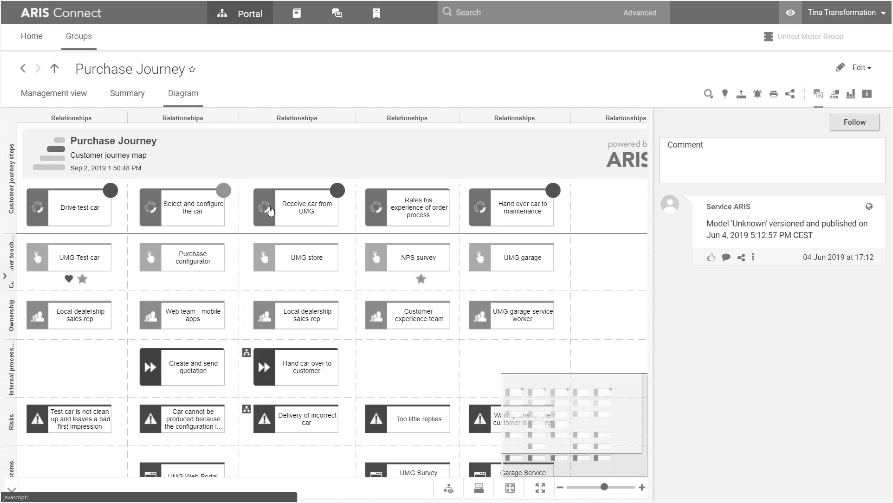
\includegraphics[scale=0.55]{DISSER-32.png}
    }
    \caption{Пользовательский интерфейс системы ARIS Platform}\label{fig:ARIS}
\end{figure}

\subsection{Инструмент системного анализа и проектирования StarUML}\label{sec:ch1/sec6/sub3}
Это программный инструмент визуального моделирования с открытым исходным кодом, который поддерживает стандартизованный язык графического описания UML для моделирования систем и программного обеспечения.
Программный продукт StarUML  от разработчика MKLabs предназначен для создания и применения графических моделей в нотации UML. Система основана на UML 2. 0 и предоставляет одинадцать различных видов диаграмм, активно поддерживая таким образом подход построения архитектур на базе моделей. Система может эффективно применяться системными аналитиками, проектировщиками и архитекторами систем, инженерами-программистами.
Программное обеспечение StarUML отличается высокой настраиваемостью в соответствии с пользовательской средой и высокой расширяемостью в своей функциональности. Использование StarUML обеспечивает высокую производительность и качество программных проектов.
Пользовательский интерфейс системы представлен на Рисунке ~\cref{fig:StarUML}.
\begin{figure}[ht1]
    \centerfloat{
        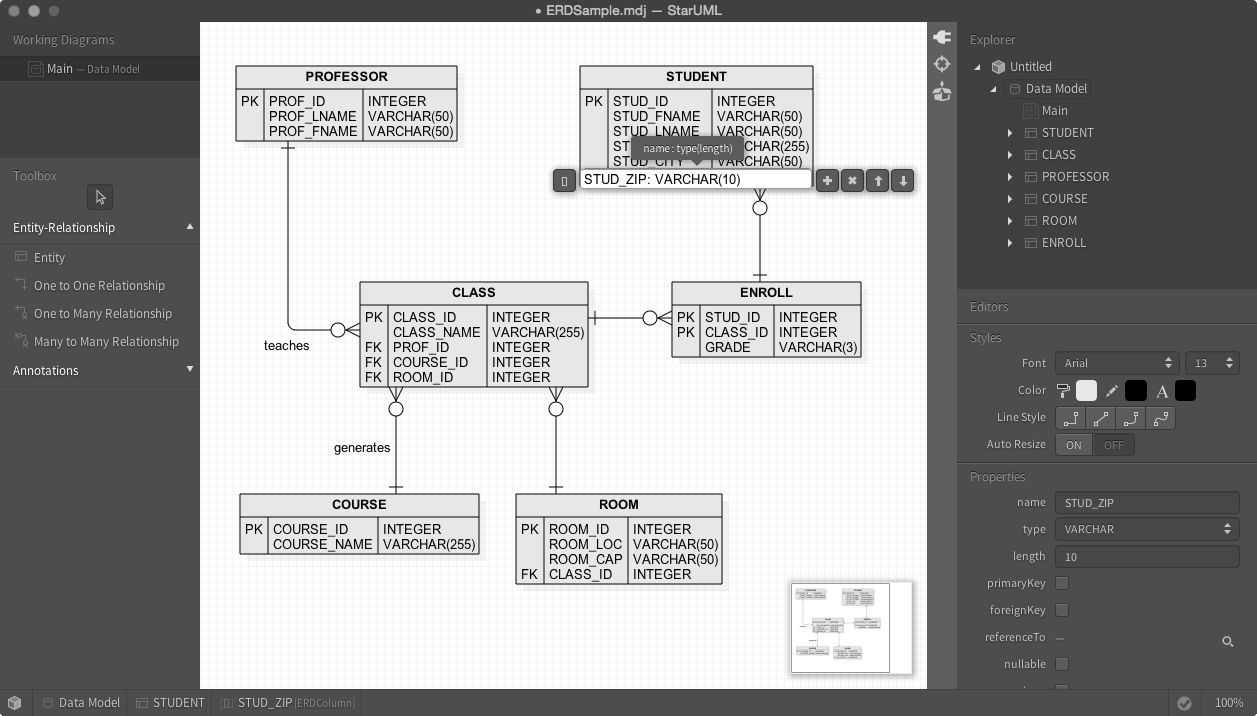
\includegraphics[scale=0.4]{DISSER-33.png}
    }
    \caption{Пользовательский интерфейс системы StarUML}\label{fig:StarUML}
\end{figure}

\subsection{Инструмент системного анализа и проектирования UNICOM System Architect}\label{sec:ch1/sec6/sub4}
Это комплексный программный инструмент бизнес и системного моделирования, позволяющий реализовывать в различных нотациях графические представления системы, требования к продукту и процесс проектирования и разработки программного обеспечения.
Программный продукт System Architect от компании-разработчика UNICOM прдназначен для визуального моделирования с целью снижения сложности предметной области и создаваемых систем, помогая более эффективно понимать сложные объекты и взаимодействовать в команде. Система UNICOM SA также помогает управлять рисками и соблюдением требований, одновременно повышая производительность и качество программных приложений и сервисов.
Пользовательский интерфейс системы представлен на Рисунке ~\cref{fig:UNICOM}.
\begin{figure}[ht1]
    \centerfloat{
        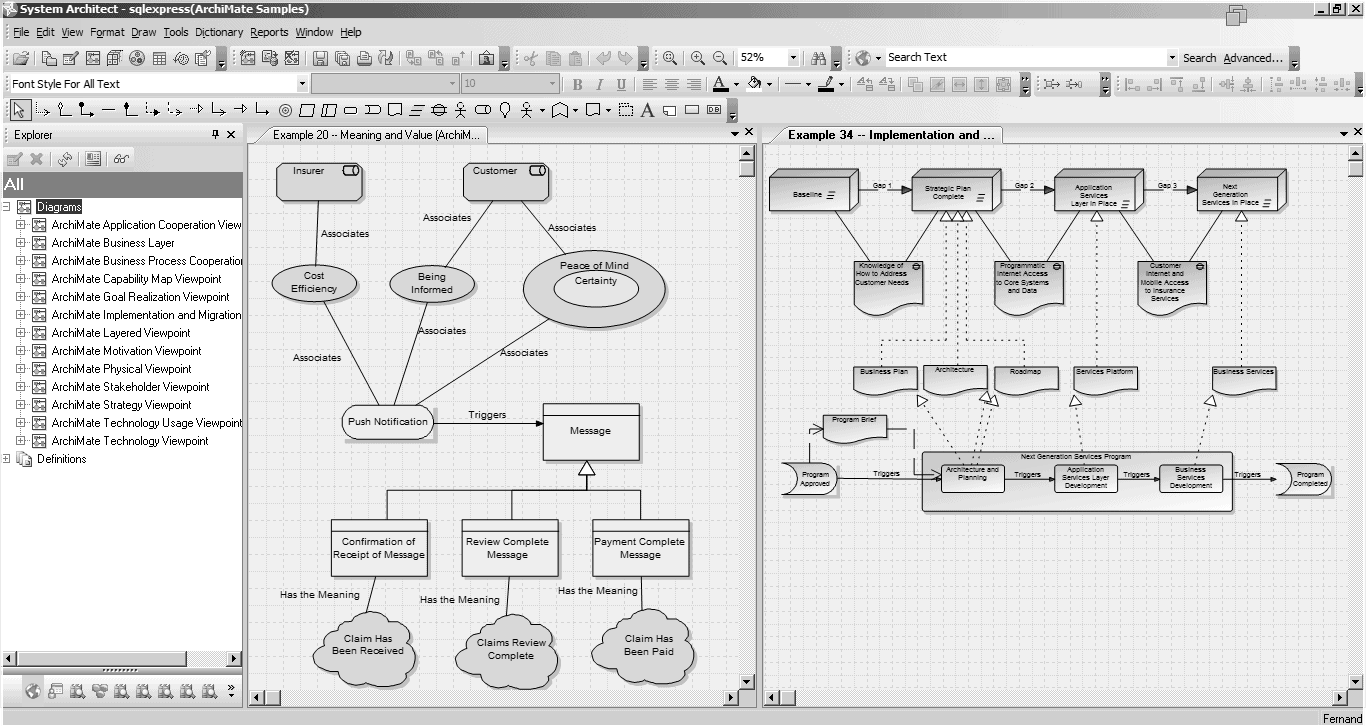
\includegraphics[scale=0.35]{DISSER-34.png}
    }
    \caption{Пользовательский интерфейс системы UNICOM System Architect}\label{fig:UNICOM}
\end{figure}

\subsection{Инструмент системного анализа и проектирования Microsoft Visio}\label{sec:ch1/sec6/sub5}
Инструменты Visio позволяют создавать диаграммы в один клик – перед этим достаточно внести все необходимые данные, и вы легко выполните нужную задачу. Программа позволяет предоставить информацию из готовой диаграммы – это делается с помощью формирования определенного отчета.
Приложение позволяет создавать чертежи, которые отличаются очень высоким уровнем информативности. Здесь используются различные элементы. Для каждой части чертежа составляются подробные комментарии.
Microsoft Visio позволяет выполнять масштабирование проекта. В качестве основы для построения схем могут использоваться системы для автоматического проектирования. Приложение предусматривает создание интерактивных панелей, которые могут использоваться для различных показателей.
Пользователи могут выполнять экспорт и импорт данных, который осуществляется между программами, входящими в пакет Office. Это увеличивает уровень удобства при работе с приложением. В программе также предусмотрена возможность для получения справки по работе с Visio. Здесь содержатся специальные подсказки и советы.
Пользовательский интерфейс системы представлен на Рисунке ~\cref{fig:Visio}.
\begin{figure}[ht1]
    \centerfloat{
        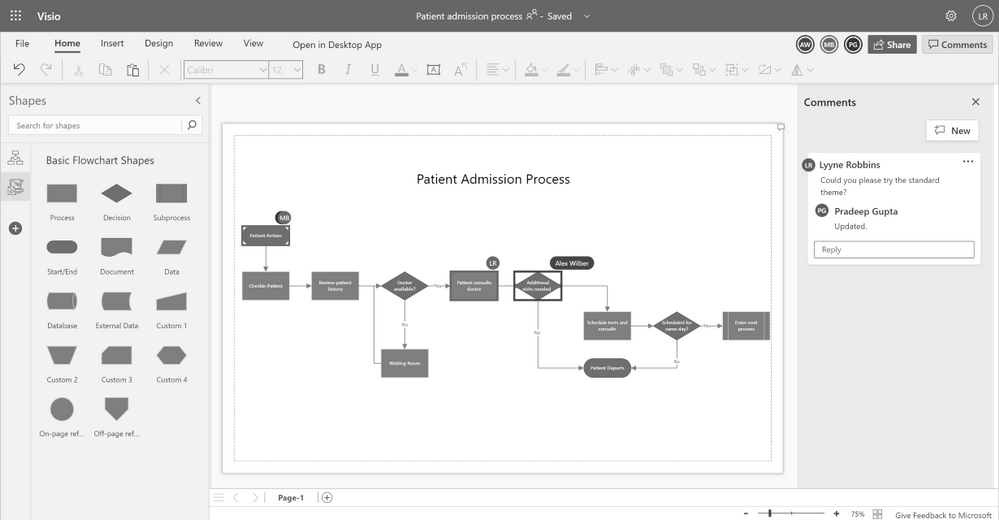
\includegraphics[scale=0.7]{DISSER-35.png}
    }
    \caption{Пользовательский интерфейс системы Microsoft Visio}\label{fig:Visio}
\end{figure}
\subsection{Инструмент системного анализа и проектирования Draw.io или Diagrams.net}\label{sec:ch1/sec6/sub6}
Это программа для управления требованиями, позволяющая предприятию любого размера создавать документы с требованиями, варианты использования и диаграммы. Программа позволяет создавать модели представления данных во всех нотациях, таких как, IDEF0, IDEF3, EPC, DFD, UML, ERD, PFDD. Существует, как облачная, так и standalone версии. Позволяет проектировать и рисовать схемы, диаграммы, бизнес-макеты, отношения между сущностями, программные блоки систем, а также элементы дизайна интерфейса программного обеспечения. В программе существует возможность добавлять палитру шаблонов для проектирования систем, согласно типам нотаций. Существует возможность экспортировать результаты работы в форматы: JPG, PNG, SVG, VDSX; программа поддерживает совместную работу: для экспорта чертежей сушествует формат .drawio, совместимый со всеми версиями программного продукта. Сервис поддерживает множество языков.
Пользовательский интерфейс системы представлен на Рисунке ~\cref{fig:Draw.io}.
\begin{figure}[ht1]
    \centerfloat{
        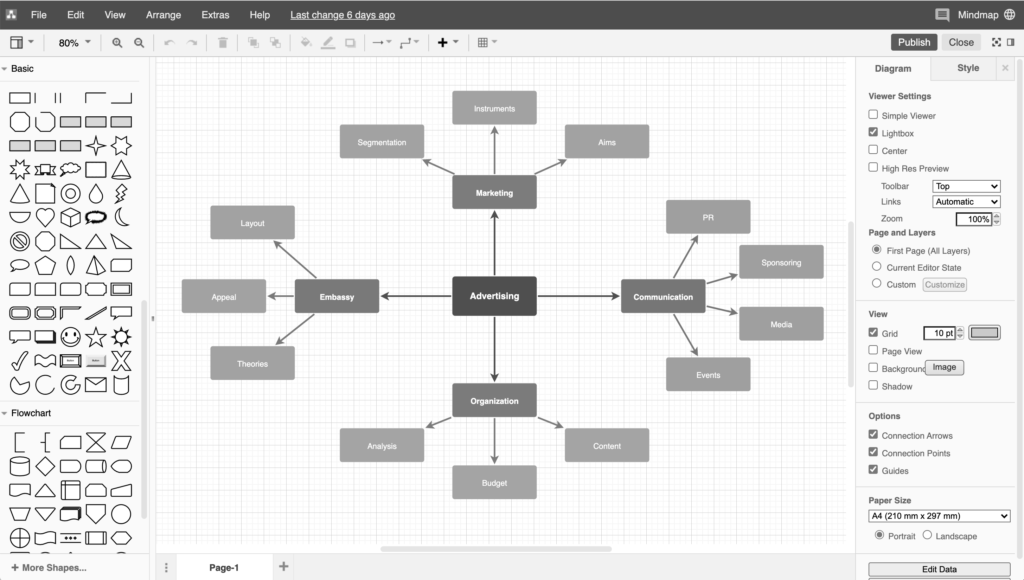
\includegraphics[scale=0.5]{DISSER-36.png}
    }
    \caption{Пользовательский интерфейс системы Draw.io или Diagrams.net}\label{fig:Draw.io}
\end{figure}

\subsection{Другие примеры}
Программ, которые помогают именно в проектировании архитектуры программного обеспечения на сегодняшний день на рынке не представлено. В основном, программы проектирования программного обеспечения предоставляют функционал по созданию: схем и чертежей в различных нотациях, графические представления системы, требования к продукту и процесс проектирования и разработки программного обеспечения. Таким образом, на данный момент явных аналогов системы не представлено.

\section{Выводы по главе}\label{sec:ch1/conc}
При проектированнии программного обеспечения среди профессиональных специалистов в этой области зачастую не хватает опыта для реализации оптимальной архитектуры программного обеспечения. Данный феномен может быть связан с различными факторами:  нехватки опыта, времени, кадров и т.д. Для того, чтобы узнать причины допущения ошибок при проектировании следует провести отдельное исследование, к данной работе этот вопрос не относится. В этой работе изучается вопрос построения системы поддержки принятия решений для проектирования архитектуры программного обеспечния. Автор работы не располагает сведениями и не изучает вопрос причин возникновения ошибок при проектировании программного обеспечения.
В данной главе был проведен обзор и систематизация основных проблем проектирования программного обеспечения. Была рассмотрена систе проектирования как полезная функция комбинации альтернатив инструментов реализации программного обеспечения. Рассмотрены наиболее распространенные инструменты проектирования программного обеспечния. Дано обоснование актуальности разработки систем поддержки принятия решений при проектировании архитектуры программного обеспечения.
\clearpage
